\documentclass[11pt, oneside]{article}   	
\usepackage[margin = 1 in]{geometry}                		
\geometry{letterpaper}                   		
%\usepackage[parfill]{parskip}    		% Activate to begin paragraphs with an empty line rather than an indent
\usepackage{graphicx}				
\usepackage{setspace}								
\usepackage{amssymb}
\doublespacing
\geometry{footnotesep=2\baselineskip}
\usepackage{longtable}
\usepackage{caption} %Put caption* in a table to remove the enumeration
\usepackage{rotating} % To rotate the reviewer table
\usepackage[numbers]{natbib}   %activates bibliography
\usepackage [english]{babel} %something for bibliography
\usepackage{verbatim} %to be able to use \begin{comment}

\usepackage{float} %fuck does this do
\begin{document}

%%%% Managerial
% Add F-tests for price
% Change Black to black? 
% Change White to white?
% Check that bibliography citations line up with their references

%%%% Writing
% CHECK LIT REVIEW IS SANE


\title{Discrimination in Airbnb: Do Minority Hosts Earn Less than White Hosts on the Platform?}
\author{Anya Marchenko}
\maketitle

\begin{abstract}

Using previously unexploited data from a large webscrape of the Airbnb website, I measure the extent of anti-host discrimination on Airbnb. I estimate that black hosts earn \$5-\$7 less per night, and Asian hosts \$6-\$9 less per night (the exact loss varies by the sex of the host), than White hosts who post a similar type of listing on the platform. I then explore various hypotheses for this effect. There is little evidence that these price disparities are due to supply-side effects, rather than demand-side effects consistent with discrimination.  For example, minority hosts are not choosing to price their listings lower, or offering their listing up for rent for shorter periods of time than White hosts. I also find little evidence that this effect is due to minority hosts owning listings of worse quality. Overall, among the hypotheses I test, discrimination is the most convincing explanation for the persistent price disparity between minority hosts and White hosts on Airbnb.\footnote{I thank Steven D. Levitt for valuable advice. Victor Lima, Kotaro Yoshida, and Ezra Karger for helpful guidance. Mahathi Ayyagari, Melody Jih, Fong Chai, Lydia Sum, Joseph Day, Leah Umanskiy, Cristian Raygoza, Putter Thepkanjana, Spencer Kang, and Tony Song provided excellent research assistance. Sylvia Klosin, Jacob Dorn, Kirthi Bellamkonda, and Michal Dzitko provided comments and feedback. Data was provided by InsideAirbnb.com, founded and maintained by Murray Cox. Sentiment analysis would not be possible without Sentimentr and coding by Ben Chaimberg.} \end{abstract}

\doublespacing
\section{Introduction} %%%%%%%%%

Over the past 10 years, sharing economies have risen rapidly as substitutes to well-established firms in the housing, car rental, taxi, and other markets. In these traditional markets, providing a good or service often has high barriers to entry, requiring compliance with extensive regulation and initial capital investment. Since sharing economies exploit the under-utilization of physical assets agents already own, participation in these new markets has far lower barriers to entry while providing an employment opportunity for agents on an at-will basis.\cite{sharing} 

As more people have entered these new markets, they have become increasingly dependent on the supplementary income they provide. Hosting with Airbnb, a platform that allows people to rent out their apartment, house, or single room to short-term lodgers, is one such opportunity. A 2017 report released by Airbnb states that in rural areas, hosts get as much as 5 - 20\% of their income from their listing.\cite{rural} Airbnb's fastest growing demographic of hosts, women over 60 years of age, earn \$6,000 a year on average from hosting, often relying on that income to supplement retirement savings.\cite{elderly}\cite{nyt2} 

%Some residents of areas of New York City have started relying on hosting with Airbnb to pay for rent or fund retirement. \cite{nyt1} 

The extent to which hosts have grown to rely on Airbnb as a source of income makes discrimination on the platform a relevant topic of research. The economic consequences of discrimination are substantial - hosts who are discriminated against would face lower demand, have higher vacancies, and earn less revenue from their listing. While one previous paper found evidence of discrimination against New York City hosts using data from 2013, no other more recent or comprehensive research has been done on this type of discrimination on Airbnb. 

% it ties into racial discrepancies in housing widely observed by economists and other social scientists. The average Black household has less mean wealth than a White household.\cite{oliver} Even when Black and Hispanic households are in the middle-class, they still live in neighborhoods with median incomes similar to those of very poor White neighborhoods.\cite{reardon} Residential preferences, differences in family structure, availability of affordable housing, and lingering racial discrimination in the housing market contribute to these disparities.\cite{krysan}  All of these long-standing factors likely affect the prices and revenues for minority hosts on Airbnb, 

In this paper, I empirically investigate the existence and extent of anti-host discrimination in Airbnb. I start by measuring the effect of host race and sex on the price of the listing and on a constructed measure of host revenue. I use data from a webscrape of around 70,000 Airbnb listings across 7 U.S. cities.\footnote{The scrape includes all of the property, host, and review information on a listing profile. To see what information would be available, see Figures 1-5 for screenshots of a sample listing. All of the information seen on the sample listing is included as variables in the data set.} For each of the 70,000 listings, the race, sex, and age of the host from their profile picture was coded. 

First, I find that non-White hosts, both male and female, across the board charge lower prices than White hosts. The biggest effect is for Asian female hosts, whose prices are roughly \$9 less per day than White male hosts who own the same type of listing. The second biggest effect is for Black males, with a coefficient of \$7, followed by Black women and Asian men with coefficients of \$6 per day, and Hispanic females with a coefficient of \$5.\footnote{This effect is statistically significant at the p $<$ .001 level for Black hosts and Asian women, the p $<$ .01 level for Asian male hosts, and p $<$ .05 level for Hispanic women.} For Hispanic men the effect is small, around \$2, and is not statistically significant.
    
Next, I construct a measure of host revenue by multiplying the price a host charges by the total number of reviews for that listing (a proxy for the quantity demanded). Using this measure of revenue, I estimate that White female hosts, Black male hosts, Black female hosts, and Asian female hosts lose about \$100-\$300 in revenue over the course of a year as compared to White male hosts who own similar listings. The exact revenue loss depends on the coefficients on price and number of reviews of a particular host.\footnote{See Table 5 and Section 3.2 for the exact effects on revenue.} These effects are statistically significant at the p $<$ .05 level or higher, and significant at the p $<$ .001 level for White females and Black females. There are also negative effects on revenue for Hispanic hosts and Asian males, but they are not significant. In Section 4, I also conduct several robustness checks and show that these results hold across various cities, price ranges, time on the market, and property types.\footnote{See Tables 6, 7 and discussion in Section 4.}

In Section 5, I consider three mechanisms, in addition to discrimination, that would explain lower prices for minority hosts: that minority hosts \textit{choose} to price their listings lower than White hosts, that minority hosts offer up their listing for fewer days out of the month than White hosts, and that minority hosts have listings of worse quality than White hosts. 

To test the first hypothesis, I consider the number of reviews that a host has as a proxy for quantity demanded of that listing. If minority hosts earn less than their White counterparts, then the opportunity cost of their time is lower. They would therefore have a lower marginal cost of putting up their listing on Airbnb and would therefore price it lower than White hosts who own similar listings. This would effectively be like their supply curve being lower at each quantity. Therefore, the quantity demanded of minority hosts' listings should be higher. To see if this is the case, I regress number of reviews as a proxy for quantity demanded on host race, controlling for my preferred specification. I find that minority hosts actually have a lower number of reviews than White hosts. This is the first piece of evidence that this supply-side hypothesis fails to explain the price disparity. The next paragraph discusses this further. Throughout this analysis, I assume that guests review hosts of different race at equal rates (for more discussion on this assumption, see Section 5, Part 1). 

To test the second hypothesis, I regress a listing's availability out of 30 days on host race, controlling for my preferred specification. A host controls how many days of the month they offer their listing up for rent via an availability calendar on the listing page. When a guest books that listing, the booked days disappear from the availability calendar. Therefore, my measure of availability is actually a measure of true vacancy of the listing. If minority hosts have lower numbers of reviews, perhaps this is because they offer their listing for fewer days of the month than White hosts. My results indicate that for Black hosts, this is not the case. The listings of Black hosts actually stay vacant on the market 1-2 days longer than the listings of White hosts. However, there is evidence that Asian hosts choose to make their listings available less frequently, which would contribute to their lower number of reviews. For more discussion, see Section 5, Part 2.      

Finally, I test my third hypothesis, that minority hosts have lower prices because they have worse listings, by looking at the quality of the reviews of the hosts. To do this, I code the demographic information of the reviewers for a randomly-chosen subset of my Chicago hosts. By having both the reviewer-side and the host-side demographic information, I can follow reviewers as they go from host to host and compare the sentiment (how favorable or unfavorable the review is) of the reviews they leave for White hosts versus minority hosts. In order to analyze the text of these reviews, I use a sentiment-analysis package in R called sentimentr.\cite{sentimentr} Rather than observing that all minority hosts uniformly had lower quality reviews, the significance of the result was either negligible or depended on the particular reviewer-host pairing. While there is some evidence that male reviewers tend to rate male hosts higher, there is little within-race preference between reviewers and hosts. Taken as a whole, minority hosts do not have lower quality reviews, as measured by my methods. For a full discussion, see Section 5, Part 3. 

I build on Edelman and Luca's research in several important ways. First, their experiment was conducted on a relatively small sample of 3,800 hosts in a single city. My sample includes seven cities throughout America, which are all large urban centers, picked so that they cover most geographic regions in the US. It is important to have this variety because discrimination in a large, cosmopolitan city with a highly diverse population such as New York might look different from discrimination in Nashville, which is more racially homogenous.\footnote{According to the U.S. Census Bureau's QuickFacts, Nashvile is 60.4\% White, 28.4\% Black, 10.0\% Hispanic, and 2.5\% Asian. New York City is 44\% White, 25.5\% Black, 12.7\% Asian, and 28.6\% Hispanic.} Second, their set of controls was limited by the relatively sparse listing information available on the Airbnb website, which in 2013 was not as comprehensive as it is today. Their covariates only included a listing's location, the number of people the listing accommodates, the rating, the number of bedrooms, and whether or not the whole apartment is available to the guest. After confirming that I get the same result when I run a regression using their controls, I then control for a more complete set of covariates.\footnote{See Table 4 for the results of my regression using their covariates. See Section 3.1 for a discussion of my controls.} Most importantly, I propose and test alternative hypotheses for these price disparities. I conclude that racial discrimination is the most likely cause for my results. 


%The covariates I add include more measures of listing size, text analyses of host-written descriptions of the listing, the time on the market of the listing, more host-specific characteristics like their response time and availability, various fees, etc. 



\subsection{About Airbnb} %%%%%%%%%%%
Airbnb is an online marketplace founded in 2008 that allows hosts to rent their private dwellings to guests as temporary accommodation. As of 2017, it has more than 3 million listings, nearly three times more than Marriott's 1.2 million rooms worldwide.\cite{aboutus} Just like traditional hotel chains, guests on Airbnb can browse listings by city and property type, and book a stay based on prices, location, past reviews, pictures of the listing, size, and amenities. Unlike traditional hotel chains, however, hosts create a profile for themselves and a page for each listing they are renting. Each listing page includes the name and picture of the host, the reviews left by previous guests, and those guests' profile pictures. Guests can therefore infer demographic information about the host through a host's picture and name, creating the opportunity for discrimination. Figures 1-5 present screenshots of a listing in Hyde Park with all of the information that would be available to a potential guest. 


\subsection{Previous Literature} %%%%%

Most relevant to this paper is the study by Harvard researchers Edelman and Luca (2014), the first to identify and measure the extent of anti-host discrimination on Airbnb.\cite{edelman} They look at the effect of host race on the price of their listing using a snapshot of roughly 3,800 New York City hosts in 2012. Controlling for several confounders that influence price, their findings indicate that non-black hosts on Airbnb have prices roughly 12\% higher than Black hosts. However, their experiment is limited by a small sample size that controlled for a narrow set of covariates. Moreover, Airbnb has since expanded and changed their website, potentially influencing the extent of discrimination on the platform. This paper addresses the limitations of Edelman and Luca's paper. I control for a more comprehensive set of covariates, which are fully outlined in Section 2.1 and Section 3.1, and also add to their work by differentiating between different mechanisms that could be driving these price disparities. 

The idea that discrimination can be reflected in prices is called market discrimination, a definition proposed by Gary Becker in his 1957 book, the \textit{Economics of Discrimination}.\cite{becker} In the Airbnb market, Becker's market discrimination would be reflected in the price that the guest (buyer) pays to the host (seller) to stay with them. If the guest is discriminating, then given two comparable listings, they would choose not to stay in the one owned by a person of color. Hosts in minority groups, responding to a lower demand, rationally post a lower price in a competitive market. If this is the case, people of color would have systematically lower prices than white males (the canonical ``default" group) for the same types of listings. 

In 1957, Becker was concerned with discrimination arising from face-to-face interactions between minority and majority groups. Since then, there has been a large amount of research indicating that Becker's theory holds for people participating in online labor, lending, rental, and other markets as well. In these cases, participants simply bring their prejudices online and use names and photos to discriminate. The canonical example is the Bertrand and Mullainathan (2004) study, which found that resumes with White sounding names received 50\% more callbacks from potential employers than identical resumes with African-American sounding names.\cite{bertrand} Doleac and Stein (2010) examined market outcomes when selling an iPod on various online marketplaces. In some pictures, a dark-skinned hand was holding the iPod, signaling a Black seller, while in others, a light-skinned hand was holding the iPod, signaling a White seller.\cite{doleac} Hands which indicates a Black seller received fewer and lower offers than White sellers. On Prosper.com, a popular peer-to-peer lending website, Pope and Sydnor (2011) find that loan listings with pictures of Black petitioners get 25-35\% fewer loans than Whites with similar credit records.\cite{pope} In sharing economies, a similar pattern occurs. Rides on Uber who use African-American sounding names end up experiencing longer wait times and more frequent cancellations than riders who use White names.\cite{knittel} A later study by Edelman and Luca (2016) found a similar result: guests with distinctively African-American names receive 16\% fewer responses from Airbnb hosts than those with White names.\cite{edelman2} These examples indicate that people often use online firms as a platform to transfer their prejudices from the real world into the online world.   



\section{Data}
\subsection{Source} %%%%%%%%%

My data are taken from the website Inside Airbnb, which provides cleaned and aggregated data on Airbnb listings in 43 cities across the world.\cite{insideairbnb} The data provided on the website are sourced from a webscrape of publicly available information on the Airbnb website. Inside Airbnb is not run by or affiliated with Airbnb itself.\footnote{Airbnb's host profiles and listings are publicly available information, and no private data was accessed in the scrape. The cleaned data is under a Creative Commons Public Domain Dedication.} The intent of the website is to inform the public on how Airbnb competes with the residential housing market in their areas. 

The scrape of the Airbnb website was conducted throughout 2015, and provides a point-in-time snapshot of all of the listings available in a particular city. This includes all of the information that would be available to an Airbnb user browsing through listings at the time of the scrape. 

Inside Airbnb provides some time-series information on prices, but since the each listing's price was not scraped daily, there are often week-long or month-long gaps in the time-series price data. A cursory glance at the time-series prices reveals that hosts do not change prices often, and if they do, they often reflect predictable weekend or holiday seasonality. There is therefore reason to believe that the prices posted at the time of the scrape are representative of the price of that listing throughout the year. However, because of the incompleteness of the time-series data set, I focus on the cross-sectional data for my main analysis.  

The variables most relevant for my analysis included in the data set are enumerated below. Each variable is per listing. 

\singlespacing
\begin{enumerate}
\item Price (including per day \& per month price)
\item Location (Includes the city, the neighborhood, e.g. ``Hyde Park", and also as a latitude/longitude)
\item Text of host-written summary of listing, listing description, transportation details, notes

\item Host-specific characteristics
\begin{enumerate}
\item Host picture 
\item Host name
\item Host availability out of 30 and 60 days
\item Number of listings owned by host
\item Response rate
\item Acceptance rate
\item Whether the host is a Superhost
\item Host cancellation policy
\item Whether host identity is verified 
\end{enumerate}

\item Listing-specific characteristics
\begin{enumerate}
\item Number of bedrooms and bathrooms
\item Square-feet
\item Type of property (apartment, house, igloo)
\item Bed type (couch, full bed)
\item List of amenities (shampoo, TV, etc)
\item Extra fees (Cleaning fees, fees for extra people)
\end{enumerate}

\item Review Information
\begin{enumerate}
\item Text of all reviews
\item Numerical review score
\item Total number of reviews
\item Picture of each reviewer
\item Date of first review and last review
\end{enumerate}
\end{enumerate}
\doublespacing

According to the website, the neighborhood for each listing wasn't pulled directly from Airbnb ``due to inaccuracies", but were identified by the scraper by comparing the geographic coordinates of a listing with a city's definition of neighborhoods.\footnote{Location information for listings is anonymized by Airbnb, and no exact address is provided for any listing. The location for a listing could be 0-150 meters from the actual address.} Figure 6 presents a map of Chicago's neighborhoods to give the reader a sense of the granularity of the neighborhood controls. 

Airbnb does not provide the demographic information of their users, so research assistants manually coded the hosts' demographic information for this paper. RAs were provided a link to the host profile picture and host name, and coded each picture according to the host's sex, race, and age. Only single-person pictures with identifiably White, Black, Asian, or Hispanic hosts were included in the main analysis.\footnote{See Table 1 for the full set of demographic categories according to which hosts were coded.} All other types of profile pictures, including couples, groups of more than two people, children, pictures without a human face, or hosts of ambiguous race were not included in the main analysis. Importantly, listings that no longer existed at the time of coding were also excluded. If hosts dropped out of the Airbnb market between the time of the scrape and the time of the coding non-randomly, this could bias the results. However, there is no way to check the demographics of the hosts who dropped out, since it is no longer possible to access Airbnb's link to their profile picture. 

Each RA was compensated based on the quantity of the listings they coded. This could create the incentive to code for speed rather than accuracy, so a simple double-checking process was put in place to check codings. For hosts whose picture was ambiguous on any of the dimensions of race, sex, or age, RAs were instructed to flag the listing. I subsequently coded each flagged picture. Since I have an incentive to code accurately in a way that RAs do not, I used this method to check RA work. Due to manpower constraints, one RA coded each picture.\footnote{It is important to note that the coding does not need to reflect the actual demographics of the host, rather, the race, sex, and age that the average person would assume to them be after looking at the picture. However, one limitation of this method is that the average University of Chicago undergraduate might not be representative of the average guest on Airbnb. With more resources, a more rigorous coding process could have been conducted. In future research, two people can code each picture, and if any disagreement occurs, have a third settle the dispute.}

A total of 70,000 host pictures across seven US cities were coded - Chicago, Los Angeles, New York City, Austin, Washington, D.C., and New Orleans.\footnote{For every city but New York, every single Airbnb listing that existed in that city at the time of the scrape was coded. In New York, which had the most listings in the sample, half of the existing 40,000 listings were randomly chosen to be coded. Time, effort, and monetary constraints prohibited the coding of all 16 US cities whose data was available on InsideAirbnb.com.} Cities with a large population, racial diversity, and geographic dispersion were chosen. This approach limits the applicability of my findings to urban areas, discounting the roughly fifth of Airbnb's listings which are located in rural areas.\footnote{A 2017 report released by Airbnb stated that 18.4\% of all active listings are located in rural areas, and there was 138\% year-in-year growth in Airbnb guest arrivals at rural listings.} In addition to main host data, demographic data was also coded for 16,000 reviewers who stayed with a subset of the Chicago hosts.\footnote{This represents about 23\% of the total number of reviewers in Chicago. Not all reviewers could be coded due to time and manpower constraints. A random subset of Chicago hosts was chosen such that the 16,000 reviews represent all of the reviews left for those hosts. Each review has a unique reviewer id, host id, listing id, the date of the review, the review text, and the coded race, sex, and age of the reviewer.} For those hosts in Chicago, it is thus possible to study the interaction of reviewer demographics, host demographics, and review quality. In Section 5, I use this data to test the hypothesis that minority hosts have lower prices because they have worse reviews. 



\subsection{Data Summary} %%%%%%

Summary statistics of host demographic information and their listings are displayed in Table 2. There is significant variation in both sex and race of the hosts on Airbnb. Single females make up 38\%, and single males 31\%, of the hosts in my sample.\footnote{23\% of the sample are couples, and the other 8\% are groups $>$ 2 or pictures without a face. These categories were not included in the final analysis.} 64\% of the hosts in the sample are White, 7\% are Black, 5\% are Hispanic, and 9\% are Asian.\footnote{The rest of the profile pictures were either pictures of groups, pictures without a human face, or multiracial couples, all of which were put in the ``Unknown/Multiracial" category in Table 2.} Black hosts in the sample are underrepresented relative to the proportion of African-Americans in the national population (about 13\% of the national population is African-American), while Hispanic hosts are underrepresented by about three times in this sample relative to the proportion of Hispanics in the population (16\%). One explanation for this could be that people self-identify as Hispanic for census data, while Airbnb hosts were identified by RAs who might have mistakenly coded Hispanic hosts as other categories. Asian-Americans are overrepresented in my sample by a few percentage points relative to the 5.6\% of Asian-Americans in the national average.\cite{census} 

The listing prices of Whites are overwhelmingly higher than any other host. The mean price of a listing owned by a white host is \$178 per night, down to \$125 per night for Black hosts, \$160 per night for Hispanic hosts, and \$131 per night for Asian hosts. Minority hosts also have lower median prices and lower standard deviations, indicating that not only do minority hosts own more cheaper listings on average, but their listings are more concentrated around the lower mean.\footnote{The median price of a listing owned by a White hosts is \$115 per night, \$90 for Black hosts, \$99 for Hispanic hosts, and \$90 for Asian hosts.} 

It is reasonable to expect that a large portion of the price differences described above are driven by differences in property characteristics. Table 2's \textit{Listing characteristics} shows that White hosts dominate the most expensive option in every single category of observable property characteristics. White hosts own the most high-priced properties (houses) and the fewest low-priced ones (apartments/lofts). They have the most bedrooms, bathrooms, beds, and amenities in their properties, and lease out more of their property than minority hosts do. In most of these measures of property quality, the listings owned by Hispanic hosts come the closest in quality to White hosts, often only a few percentage points behind. Either Black or Asian hosts have properties of the lowest quality as measured by these metrics, depending on the category. 

While White hosts do well and Black hosts lose out in property characteristics, this is not the case for host characteristics. In categories where the host can influence their desirability by being ``a better host" by responding on time, putting in effort into writing longer descriptions, or making their listing available for more days out of the month, Black host do well. They have the highest response rate at 77\%, with White and Hispanic hosts behind them at 75.6\%. They make their listings available 14 days out of the month, a full 4 days more than White hosts. However, Black hosts have the lowest acceptance rate, accepting only 36\% of guests who ask to stay with them. Hispanic hosts have the highest acceptance rate at nearly 50\%. 

Black and Hispanic hosts also do well in some of my constructed measures of ``host quality". They describe their listings using  as many or more good words like ``airy", ``beautiful", and ``clean", an average of .04 words higher than White hosts. While White hosts write the longest descriptions in every host-written field, Black hosts are, on average, only four words behind White hosts in this metric. Asian hosts write the shortest descriptions in every host written field. The difference between White and Asian hosts increases as the fields get less prominent on the profile. At most the difference in the length of descriptions that White and Asian hosts write is 13 words, or approximately the length of a short sentence. See Figure 2 for an example of host-written descriptions on a real listing profile. 

White hosts also have the highest number of reviews, and the highest review ratings. Since Airbnb assigns Superhost status based on the number of stays a host has, the quality of the reviews, and their response rate, it is not surprising that White hosts also have the most Superhosts: 13.4\% of White hosts are Superhosts, while the next runner-up, Hispanic hosts, are at 10.8\% Superhosts. 

The reviewers who stayed with the Chicago hosts have similar gender diversity as the overall host population but significantly less racial diversity. Roughly 33\% of the reviewers are female and a similar proportion is male. However, 67\% of reviewers are White, with only 6\% being African American and Hispanic (about 500 reviewers each), and 12\% Asian. Importantly, the measure of review quality externally assigned by Sentimentr to the text of each review generally matches up with the numeric scores reviewers gave. While all hosts have on average very positive reviews, White hosts have the most positive review sentiment, followed by Hispanic, Asian, and Black hosts, but the differences between them are not significant. 



















\section{Results}
\subsection{Main result: Do minority hosts have lower prices than White hosts?} %%%%%%%%%%%%%%%%%

Before analysis, the data set used was restricted to hosts who have profile pictures and manage less than 20 listings, and listings priced at less than \$800 per night. 64,611 listings were left after restricting the data set. There were only 20 hosts who did not have profile pictures, so in the case that minority hosts, expecting discrimination, did not include a picture, there is little chance that dropping hosts without a picture biased my results. 

Table 3 presents OLS estimates of the effect of host race and gender on the listing price. The specification is of the form: 

\[ Price_{i,j} = Race_{j}\,X \,Sex_j + Age_j + x_{i,j}\]

The $Price_{i,j}$ is host $i$'s price from their Airbnb listing $j$. For hosts with multiple listings, each listing is treated separately. The $Race_{j}\,X \,Sex_j$ is the interaction of the race and sex of the host. White males are the omitted category. $Age_j$ is the age of the host (young, middle-aged, or senior). Young hosts are the omitted category for age. $x_{i,j}$ is vector of other covariates that increases from left to right in the columns of Table 3. The columns are additive in their covariates, so each column controls for everything in the previous columns, plus its new set of covariates. Standard errors are clustered by neighborhood throughout, thereby allowing for listing prices to be correlated in a particular neighborhood.

The first column, Model 1, in Table 3 presents just the raw effect of host race and sex on the price of a listing, not including any covariates. These are consistent with the mean listing prices by race presented in Table 2, except now also broken down by male and female hosts within each racial category.

\textbf{Model 2: Addition of location controls}

Model 2 adds city and neighborhood fixed effects.\footnote{Neighborhoods are assigned in accordance with each city's designations} In Chicago, for example, the fixed effect granularity is at the level of locating a listing within Hyde Park vs. Woodlawn. Location is an important proxy for income levels, crime rates, and distance from downtown, which are all predictors of property prices and therefore listing prices on Airbnb. As expected, controlling for location substantially decreases the estimated racial gaps in prices. The coefficients for minority hosts decrease from a range of \$20-40 to a range of \$10-20 (these are all negative, and relative to White male hosts). I observe the largest decrease in the coefficients on Black hosts, which go down from \$40 to roughly \$15. Coefficients of Hispanic hosts decrease by around \$10; Asian hosts by about \$20. 

It is well-documented that blacks in urban populations are nearly four times more likely than Whites to live in neighborhoods where the poverty rate is 40\% or higher.\cite{firebaugh} In fact, minorities at every income level live in poorer neighborhoods than do Whites with comparable incomes. For example, a Black household earning \$75,000 a year resides in a higher-poverty neighborhood than a White household with earnings of less than \$40,000 a year.\cite{logan} It is therefore expected that a large part of the variation in Airbnb prices between those groups can be explained by their listing's location. The coefficients of White females, on the other hand, persist at around \$4 with the addition of location controls. This is most likely because White females tend to live in the same areas as White males and therefore have little to no variation in price that can be explained by differences in neighborhood.  

\textbf{Model 3: Addition of property controls}

Model 3 adds controls for listing-specific characteristics. Listing characteristics added include fixed effects for the property type (house, apartment, etc) and the room type, the time the listing has been on the market (as proxied by fixed effects for the month and year of the listing's first review), number of guests the listing accommodates, the number of bathrooms, bedrooms, and beds, the bed type (couch, full bed, etc), the number of amenities, the number of minimum nights, any fees for cleaning or extra people, whether the listing is instantly bookable, and the cancellation policy. Controlling for these listing characteristics decreases all effects to \$5-10, depending on the race of the host. Asian female hosts had the largest decrease in coefficient after controlling for listing characteristics, which indicates that a substantial part of their effect was driven by owning properties with worse observable characteristics. The effects for Hispanic males and White women disappear with the addition of property controls - while they are slightly negative, they are not significant. The effects on middle-aged and senior hosts are almost eliminated by controlling for property characteristics, indicating that their higher listing prices are primarily driven by better observable characteristics. 

In general, from Model 1 to Model 3, coefficients steadily decrease and $R^2$ increases from .166 with neighborhood controls to .621 with property controls. Most of the variation in price between minority hosts and White male hosts can be explained by either the property's location or observable property characteristics. The $R^2$ jumps substantially to .621 in Model 3, so adding property characteristics explains much more of the total price variation than the location. This might be because Airbnb listings tend to be more concentrated in certain areas of each city (North side in Chicago, lower and middle Manhattan in New York City, etc). If listings in a city cluster together instead of being uniformly dispersed, then controlling for location won't explain as much of the variation as controlling for property characteristics.   

\textbf{Model 4, final specification: Addition of host \& quality controls}

The last column presents my full, preferred specification. It adds host-specific characteristics to Model 3, including the host response time and the host response rate, whether the host is a Superhost (Airbnb's special designation for highly-rated and popular hosts), whether the host identity was verified by Airbnb, and if the host requires a guest's profile picture or phone to book. 

Importantly, Model 4 also controls for variation in host effort. I attempt to account for the idea that some hosts may have higher prices not because of better observable characteristics, but just because they are better hosts. There are several host-written fields on each listing page, the ``Summary", ``Description", ``Space", ``Neighborhood Overview", ``Transit", and ``Notes". By filling out these fields, hosts not only describe their listing, but have the opportunity to provide guests with helpful tips and information about the surrounding area. How well a host writes these descriptions is therefore a reasonable proxy for how much effort they are willing to put into hosting. To this end, I construct three variables to measure host effort. My first variable simply measures the length of each of these fields. Presumably, the longer the description, the more effort the host put into writing it. My second variable measures whether these fields had mostly long words or short words, so that a description that uses shorter words, such as ``My house is nice", would be counted as lower quality than ``My house is gorgeous". 

My third measure of host effort is a rudimentary sentiment analysis of the ``Description" field. Hu and Liu (2004) create a list of 2,006 positive words that commonly appear in customer reviews to aid in sentiment categorization.\cite{hu} I take 7 positive words from their list that would be most relevant for Airbnb listings: ``spacious", ``beautiful", ``clean", ``comfort", ``great", ``love", and ``quiet". I only include words that have substantial variation in the description, meaning that more than 5\% of descriptions had these words. This narrowed the list of viable words significantly. I then added a covariate for the number of these ``good words" in the host's ``Description" field. Together, these three ``host effort" variables control for hosts who write longer descriptions, use longer words in those descriptions, and put more words that are associated with positive reviews in their descriptions. 

\textbf{Discussion}

After controlling for my final specification, I estimate that, across the board, minority hosts earn lower prices from their Airbnb listing than White hosts. The biggest effect is for Asian female hosts, whose prices are roughly \$9 less per day than White male hosts who own the same type of listing. The second biggest effect is for Black males, with a coefficient of \$7. The coefficients on Black women and Asian men are \$6 per day each, Hispanic females is \$5. This effect is statistically significant at the p $<$ .001 level for Black hosts and Asian women, the p $<$ .01 level for Asian male hosts, and p $<$ .05 level for Hispanic women. For Hispanic men the effect is around \$2 and is not statistically significant. There is little effect for White females, and a small effect that's not statistically significant for middle-aged and senior hosts. An F-test shows that host race is jointly significant for price at the 0.00 level after controlling for both Model 3 and Model 4. My results are stable to the addition of host characteristic controls. These effects are robust to clustering standard errors at the neighborhood level. The inclusion of these host characteristics does not improve the fit of the model substantially. Property characteristics and location still explain more of the variation in price than host characteristics. 

My results are consistent with Edelman and Luca's findings, but I find smaller effects (they found a 12\% price disparity, I found about a 7\% price disparity). This is most likely because I control for a larger set of covariates. To confirm this, I run a regression on listings in New York City, controlling for the same covariates that Edelman and Luca used in their main result. The results, presented in Table 4, show that I get an almost identical coefficient as the one they found - an \$18 price difference between Black hosts and White hosts. This indicates that my main results in Table 3 were smaller because I controlled for more variation, not because of a structural change in the extent of discrimination in Airbnb.\footnote{I mimicked their set of regressors as best as possible, but because Airbnb changed their user interface in the past four years, several of their regressors I approximated with the closest variable available in my data. For example, instead of whether the host had social media accounts, I controlled for whether the host's contact information was verified by Airbnb.}

If one believed the price difference was driven by unobserved characteristics in the error term, one might have expected that the price gap between White and minority hosts would disappear with the addition of more controls. This is true up to a point, since when I add more covariates my coefficients shrink relative to Edelman and Luca's. However, after that, my coefficient of interest is stable to the addition of controls - adding host-specific controls does not substantially change any of the effects. As one might expect, the $R^2$ goes up to .621 with the addition of location and property controls, but adding my host controls increases the $R^2$ by only .006. 

If the exist, there are a few possible sources of unexplained variation in the price of the listing - variation in the real, physical qualities of the listing that wasn't captured by the property controls, and variation in the quality of the listing's profile that was not captured by the host controls. Since I was able to control for all of the property-quality variables that Airbnb offers on a listing page, it is unlikely that there are unobserved property characteristics driving the price differences. Since adding host controls explained very little variation in the price, increasing the $R^2$ by only .006, it is unlikely that adding more sophisticated measures of host quality or effort would significantly help explain price disparities. While this does not eliminate the possibility that there is a set of controls not related to property type of host type that would have increased the $R^2$ drastically, this is still good evidence to believe that the price difference I estimate is a real difference, rather than purely caused by endogeneity. 


\subsection{Secondary result: Estimate of yearly revenue loss for minority hosts}

To estimate the revenue loss that would result from the price differences found in the previous section, I construct a measure of revenue equal to: 

\[Total \: Revenue \ = \ Price \: Per \: Day \ * \ Reviews \: Per \: Month \ * \ 12\] 
%% \ and \: and \, and \quad and \qquad symbols make spaces in math mode

The estimates of the effect of host race on host revenue are in Table 5.\footnote{I acknowledge that there are potential problems associated with using number of reviews as a proxy for demand, which are briefly mentioned in the introduction. I fully discuss them in Section 5.} Consistent with my prediction, all of the estimates are negative and in the range of \$100-300 dollars. The biggest yearly revenue loss in the entire sample is for Black females at \$300, or about a 12\% loss. Black males and Asian women lose about \$160-180 throughout the year. Notably, White females, who had no statistically significant effects on their price in Table 3, have a significant revenue coefficient of \$144. This is because of reasons inherent to the definition of revenue. Even if White women didn't have a statistically significant difference in price from their male counterparts, they do have a lower number of reviews. In the next two sections, I present and discuss evidence that \textit{both} the price and the number of reviews for minority hosts are lower than for White male hosts. That means that when I multiply these two values together, two complementary effects both lower the total revenue of hosts. Overall, however, the same groups which had significantly lower prices also have lower revenues - Black males, Black females, Asian females, and White females all have significant effects in the several hundreds of dollars. 
 


\section{Robustness checks of main result} %%%%%%%%%%%

In this section, I see if my effects on price persist when I break up my data by city and property type. 

\textbf{Effects persist between large cities}

Edelman and Luca found much larger effects of host race just in New York City than I did in data that included all seven cities. A reasonable hypothesis for this is that New York City is driving all of the variation in price, and when other cities are included, where discrimination might not exist, the effects get smaller. To test this, I broke up the effects of host race on listing price by city and controlled for my preferred specification. The results are in Table 6. In general, no single large city in my data set is driving all of the variation in my data. The effects on price are mostly negative for minority hosts, with a few positive coefficients in cities with fewer observations. As expected, New York City and Los Angeles, the cities with the most host diversity and largest sample size, most closely resemble the coefficients from my main result in Table 3. In smaller cities, more than half of the negative effects are significant to various levels, and none of the positive effects are significant. 

However, there are a few outlier coefficients that are most likely driven by low sample size in smaller cities. The coefficients for Black hosts are fairly consistent with the combined data in all cities but New Orleans. In New Orleans, a Black host is estimated to earn \$18 less for the same kind of listing as a White host, an effect that is statistically significant at the p $<$ .05 level. The coefficients on Hispanic hosts are mixed - in LA, NYC, and Chicago, the coefficients on Hispanic hosts are approximately the same as the combined analysis, while in Austin, New Orleans, and DC, the coefficients are slightly positive. The outlier coefficient is in Nashville, where Hispanic hosts are estimated to earn \$39 less per day than a comparable White host. However, there are only 21 Hispanic hosts in Nashville, so this result is not very generalizable. In LA and NYC, the coefficients of Asian hosts are consistent with the combined data in sign and magnitude. However, they have large coefficients of -\$18 to \$28 in Chicago and Austin, respectively, both of which are significant. The reasoning is similar to Hispanic hosts. 

Generally speaking, the price difference in New York City and Los Angeles is relatively the same. While there are outlier coefficients in smaller cities, it is unlikely that discrimination against Asian and Hispanic hosts in those cities is actually 8 times higher than New York City or Los Angeles. Rather, those cities often have less than 50 hosts in a particular racial category, so any outliers have the potential to skew the coefficients to a much larger degree.  

\textbf{Effects persist between listing types}

Table 7 presents the effects of host race on price, broken down by various listing characteristics such as price, time on market, and property type. I break up the listings by price in the following way: separately for Los Angeles and New York City, I predict the price of a listing based on its property and host characteristics, without host race. I then use this predicted price to break up listings into higher vs. lower than the mean predicted price in those cities. I control for my preferred specification.  

I find that there is much greater price disparity between White and minority hosts among high-priced listings rather than low-priced listings. Column 1 of Table 7 considers price disparities only in listings priced below-average in Los Angeles, and Column 2 considers only above-average priced listings in Los Angeles. The price disparities are much larger for the expensive listings - \$10 for Black hosts, \$15 for Hispanic hosts, and \$18 for Asian hosts. By contrast, the coefficients are much smaller, only \$2-3, for the cheaper listings. This pattern in price disparities indicates that discrimination is more pronounced against minority hosts who own more expensive properties than against minority hosts who own cheaper properties. In New York City (Columns 3 and 4), the coefficients for expensive listings are larger than coefficients for cheap listings by about \$6, so this effect is not limited to one city or driven exclusively by city-specific characteristics. One hypothesis for this effect is that all of the discrimination is statistical, in which case the host race isn't as much as a proxy for property value for guests for cheap listings  as it is for expensive listings, which are owned primarily by White hosts. Another explanation is that if guest is expecting to put up a larger financial investment, they are more selective about which listings they stay at, so any existing discrimination is exacerbated. 

Columns 5 and 6 show that the price disparities are similar for both old and new listings (defined as listings that have been on the market more and less than two years, respectively). This suggests that the effects of discrimination are \textit{not} erased out by spending a longer time on the market; in other words, minority hosts do not simply ``catch up" to White hosts after a few years. Columns 7-9 break price disparities up by property type. The effects for Black hosts across property types get more pronounced the more expensive the property type. While Black hosts who own an apartment expect to earn \$5 less per day than White hosts, that number increases to an \$11 loss for Black hosts who own houses. This is consistent with the results in Columns 1-4 and with the statistical discrimination hypothesis - if hosts are using race as a proxy for property value, then we should expect guests to discriminate more against minority hosts who own more expensive properties, such as houses.   


\section{Testing Alternative Hypotheses}
\textbf{Hypothesis 1: Are prices lower due to supply-side effects?}

Market discrimination laid out by Becker rests on the idea that groups who are discriminated against see lower demand in the market, which drives down their prices. I have estimated that prices are lower, but there could be multiple explanations in addition to discrimination for this result. One hypothesis is that, for the same type of listing, minority hosts \textit{choose} to price their listings lower than White hosts. This might happen if minority hosts earn lower wages because they experience discrimination in the labor market. A lower opportunity cost of time would mean they have a lower marginal cost of putting up and managing their listing than a White host who owns a similar property. If minority hosts choose to price lower for every quantity, this is, in effect, equivalent to the supply curve being lower for minority hosts relative to White hosts. We therefore know that we can test this hypothesis by looking at the quantity demanded. If prices are low because the supply curve is lower, then minority hosts would have a higher quantity demanded. Conversely, if the price are low because the demand curve is lower - which would be in line with the presence of discrimination - then the quantity demanded should be lower than it is for White hosts. 

In order to test this hypothesis, I use number of reviews as a proxy for quantity demanded. In Table 6, I regress the number of reviews on host race, controlling for the same set of models as Table 3. I find that minority hosts have either the same or lower review numbers than White hosts for a similar listing that spent the same amount of time on the market. Most coefficients are either roughly zero, or negative and in the range of 1-2 reviews less than White hosts. The results are significant for White females and Black hosts. While the coefficients were significant for Asian hosts under the less robust specifications, under the full specification the coefficient is not significant, but still slightly negative. In general, my results suggest that non-White male hosts do not see a higher quantity demanded than White male hosts. This is evidence against the supply-side explanation. 

It is important to keep in mind that this conclusion is only salient if the total number of reviews is a reasonable proxy for the demand of a listing. Yet, one can imagine that if reviewers systematically under-review minority hosts relative to White hosts, these groups would have lower numbers of reviews that do not necessarily represent a lower quantity demanded. There is no way to tell apart these mechanisms in my data, and no previous research has been done on race-based differences in review rates. 

My working assumption is that even if not every guest leaves a review, the review proportion is similar across host race, and a lower number of reviews therefore indicates a real difference between quantity demanded of minority hosts and White hosts. I substantiate this assumption with another supply-side metric, a measure of listing vacancy that I explore in the next section, that provides more evidence that lower prices are not driven by supply-side effects. Taken together, these two measures will provide strong evidence to reject the hypothesis that lower prices are due to supply-side effects. 
    
    
\textbf{Hypothesis 2: Are number of reviews lower because minority hosts offer their listings a fewer number of days?}

In the previous section, I argued that minority hosts had a lower quantity demanded than comparable White hosts. However, they may have lower number of guests because they offer up their listing for fewer days of the month, not because people don't want to stay with minority hosts. In order to test this, I regress the availability of the listing out of 30 days on host race, controlling for my preferred specification. The availability of a listing is controlled by the host, who can update their availability calendar on their listing page. Potential guests can then see on which days the listing is available and book accordingly. When a guest books an available day, that day is removed from the availability calendar. Therefore, the availability out of 30 days measure is a true measure of the \textit{vacancy} rate of a listing.

The results, presented in Table 7, are striking. I find that the listings of Black hosts spend about 20\% more time on the market vacant than the listings of White males. The effect is statistically significant, and amounts to about 2-3 days per month in real units. Interestingly, White females make their listing less available than White males, with approximately a .9 of a day statistically significant difference. This might explain why White females don't have lower prices than White males, but did have lower numbers of reviews. Perhaps White females simply offer their listing for fewer days than their White male counterparts. There were no statistically significant effects in availability for Hispanic hosts, like for most of my measures. Asian female hosts actually had a lower vacancy rate than White male hosts, which could help explain why they have a lower number of reviews. 

Overall, there is strong evidence that even though Black hosts offer their listing for more days, they have less people staying with them than White hosts. This is significant evidence to reject the supply-side hypothesis for Black hosts. This is not the case for Asian hosts - the coefficients for Asian hosts were negative, indicating that they actually are putting up their listing for rent less often than White hosts. This means that lower availability is another possible explanation, in addition to discrimination, for why Asian hosts have a lower number of reviews. However, I am not able to further distinguish between these two hypotheses in my data.  

\textbf{Hypothesis 3: Are their prices lower because minority hosts have worse reviews?} 

Reviews are often critical for the decisions guests make about the listings they book. It is reasonable to expect the quality of a listing's reviews influences the demand, and therefore the price, for that listing. Previous analyses, including Edelman and Luca (2014), involved controlling for the numeric review score of the listing as a proxy for listing ``quality". However, the numeric review score on a listing often carries little information about the real quality of the listing because there is very little variation in the numeric score. In my data, 50\% of listings had an average review of $>$ 96 out of 100, and 75\% had an average review score above 91 out of 100.\footnote{This is the case for most online marketplaces. Fradkin, Grewal, and Holtz (2017) study the determinants of review informativeness on Airbnb and find that most reviews, both numeric and text, are positive. In general, reviews tend to reflect real experience of the user.\cite{fradkin}} An Airbnb guest, seeing little variation in the number of stars different hosts have, may instead rely on the text of the reviews to make their booking decision. Since review text allows guests more flexibility in the feedback they give, it may provide a more accurate and nuanced picture of the guest's experience.\footnote{This is because a guest who leaves a text review have the opportunity to use qualifiers like ``but", or ``except", strengthening words like ``really" or ``a lot", etc.} For this reason I use review text instead of the numeric score in the analysis. 

In order to do this, the race, sex, and age of 16,000 reviewers who left reviews for a subset of the Chicago hosts was coded.\footnote{16,000 is 23\% of the total amount of Chicago reviewers in the data set} For each sentence of each review, I used a sentiment-analysis algorithm called Sentimentr to evaluate how positive or negative the sentence is. Sentimentr uses a dictionary of positive and negative words to assign each sentence a sentiment score from -1 to 1, where 1 is a positive sentence, -1 is a negative sentence, and 0 is a neutral sentence carrying no emotion. Unlike other sentiment analysis programs, Sentimentr doesn't merely count the number of good or bad words in a sentence. It also takes into account valence shifters, or words that affect the sentiment-carrying word in the sentence. For example, the algorithm assigns ``I like the listing", ``I \textit{really} like the listing", and ``I like the listing, \textit{but}..." different valence scores because of the presence of valence-shifting words like ``really" and ``but". Sentimentr calculates the correct sentiment 60-70\% of the time as compared to a human grader. One limitation of conducting sentiment analysis in this way, however, is that not every review that a human would consider bad or good carries a sentiment word that the algorithm would pick up. For example, ``The apartment had cockroaches" is certainly a horrible review, but would be given a score of 0 by Sentimentr because it contains no emotion-laden words. 

In Table 8, I regress this sentiment score on the host race, controlling for my preferred specification from Model 4 in Table 3. This means that each coefficient should be read as the standardized review quality, relative to White males, that reviewer of type A gave host of type B.\footnote{Review quality was standardized with mean 0 and standard deviation of 1.} I break up my regressions by the race and sex of the reviewer, varying across the columns of Table 8. The race and sex of the host varies by row. I therefore am able to see any trends in the quality of the review different types of reviewers gave to different types of hosts. 

I find that results were mixed. Overall, White reviewers show little evidence of systematic bias against minority hosts, as measured by the sentiment scores provided by Sentimentr. The reviews that White guests leave for minority hosts do not significantly differ in quality from those they leave for White male hosts. There are stronger effects when considering the quality of the review minority reviewers gave to minority hosts. Black male guests rate Asian hosts almost 4-8 standard deviations above the mean, but rate Black women 3 standard deviation lower than the mean. All minority female reviewers, including Black females, rate Black men worse than they would rate White men who own a similar type of listing. However, all minority male reviewers rate Black men anywhere from .5-2 standard deviations higher than they do White men. This suggests that there is some gender-based favoritism between minority reviewers and Black male hosts. However, it is important to keep in mind that some of these large, very significant coefficients are suspicious because of small sample sizes - in several thousand Chicago host and reviewer pairs, there are simply not enough Black men who stayed with Asian women to be representative of the overall distribution.

In general, there is no one minority group that uniformly has lower quality reviews. Some groups do tend to give other groups far better reviews, but there is no larger pattern of within-gender or within-race bias between hosts and guests that holds for more than one host-guest pair. Overall, there is not enough evidence to substantiate that minority hosts have systematically lower review quality that can explain lower prices. 



\section{Conclusion \& Further Work}

In this paper, I estimate that minority hosts on Airbnb, especially Black and Asian hosts, earn \$5-\$9 less per day for the same type of listing as White hosts. This amounts to a yearly loss in revenue of \$100 - \$300. Importantly, I rule out several alternative hypotheses that could be driving these results, and show that racial discrimination is the explanation most consistent with my findings. 

Discrimination on the platform is pertinent as subject of research because Airbnb itself can do much to address these issues. 
In response to media outcry about allegations of discrimination, Airbnb updated its Discrimination Policy in September 2016, increasing instant bookings (the opportunity for guests to book without waiting for host approval) and making host profile pictures smaller. Evaluating Airbnb's efforts to address discrimination is therefore a relevant extension of this research. Since InsideAirbnb.com is continually being updated, there is now data available from webscrapes of listings after Airbnb's new discrimination policy took effect in September of 2016. Future work can explore whether the policy helped to curb discrimination on the platform by measuring the extent of discrimination before and after the policy took effect. If user interface really does influence the extent of discrimination in Airbnb, then the prices of minority and White hosts should start converging, suggesting that discrimination was causing the price disparities in the first place. 





\begin{comment} %%%%%%%%%%%%%%%
\section{GARBAGE SECTION: Alternative Hypotheses} %%%%%%%%%%%%%

In this section, I consider alternative explanations for the price differences I found between minority and white hosts. In particular, I examine three relevant mechanisms that are not discrimination that could explain my results. I will then argue that these mechanisms would be insufficient in doing so. 

\textbf{2. Price observed during the scrape is not the price normally set by hosts or observed by guests}

The prices I used in my data analysis were prices from one particular day in 2015-2016. I ran my regressions on the assumption that this is the price that hosts set and that guests observe that drives guest booking decisions and host revenue outcomes. However, imagine that for one day, all of the white people on Airbnb raise their prices. That day, the scrape happens to take place, and the next day, the prices of White hosts all go back down. Then, the price that I observed in my data for White hosts would be high even though it doesn't incorporate real demand differences between races nor is tied to listing characteristics or host quality. While this may seem like an unlikely scenario, price hikes for the weekend or for holidays like July 4th or New Year's may give rise to a similar situation if Black hosts change their prices differently than White hosts. 

TO-DO - Check price time series data to prove that prices don't move around that much during the month/year. 

\textbf{3. Data clean-up disproportionately dropped lower-priced listings of White hosts or higher-priced listings of minority hosts}

During my analysis, I left out hosts that had no profile picture. If hosts are aware of the potential effects of discrimination, minority hosts might be less likely to include a profile picture. If minority hosts who own higher-priced listings dropped out of the data set in this way, my coefficients might be biased downward because the sample doesn't include the higher-priced listings owned by minority hosts. A similar thing could have happened when I restricted my data set to listings with a price per night of less than \$800, and to listings owned by hosts who owned fewer than 20 listings total. If those hosts who owned a lot of listings or charged wildly high prices per night were disproportionately Black, Hispanic, or Asian, I'd see a similar downward bias on my coefficients.

TO-DO - Examine who I am dropping when I do data-clean up. 



************Garbage
After controlling for listing characteristics, host characteristics, and the neighborhood location of the Airbnb, and time on the market, I find that all host categories, but especially black male hosts, white female hosts, black female hosts, and Asian female hosts, for whom the result is statistically significant at at least the p < .01 level, earn approximately \$200 less during the course of their listing than white male hosts.  will earn \$190 - \$284 less revenue from their Airbnb over the course of the posting relative to their white male peers. The effect is statistically significant at the p < .001 level for white female and black female hosts, and significant at the p < .01 level for black male hosts and Asian female hosts. While there is a large downward effect on revenue for Hispanic male, Hispanic female, and Asian male hosts, it does not persist after controlling for listing and host characteristics. Contrary to what one would expect from discrimination literature, out of the groups for whom I could measure discrimination, black male fared the least poorly, earning \$190 less than white male hosts over the course of their listing?s lifetime. Women as a whole, regardless of race, do worse than black men. Asian women earn \$232.6 less in revenue and white women earn \$272 less in revenue than white male peers. Black women hosts fare the worst out of any of the groups considered, earning \$283.6 less than white men over the course of their Airbnb listing. 

white male reviewers gave lower reviews only to Asian female, with a .074-unit decrease relative to white male hosts. Black male guests gave white female hosts .207 units, two white male hosts .624 lower, Asian men .517 units higher quality reviews than they gave white men. White females gave lower quality reviews only to Asian women at a rate of .099 units less. Black female reviewers gave Airbnbs owned by two black women an entire valence point, 1.005 units better reviews than white male hosts, but rated Hispanic women .647 units lower. Asian females rated Black male hosts .358 units worse than white male hosts. 

 
 TO-DO: Add Levitt and Fryer? Black names paper
List (2004) found a similar result at baseball card shows, with Black sellers getting offer 3-30\% worse than White sellers. 
 
 Becker explains, ``If someone has a `taste for discrimination', he must act as if he were willing to forfeit income in order to avoid certain transactions; it is necessary to be aware of the emphasis on the words `as if'" (Becker 16).While market discrimination harms the discriminated group because it lowers their wages, taste discrimination can also harm the person discriminating, since they might now be paying more for the same good or service - whether in opportunity cost or price -  because they prefer not to interact with the discriminated group. 
Another type of discrimination laid out by Becker is taste discrimination, in which people ``prefer" not to interact with certain groups. This type of taste discrimination that is based on a general dislike could show up in the reviews that are left on host profiles. If a guest stays with a host against whom they are prejudiced, they may leave a worse review or rating, a shorter review, or no review at all, than a comparable stay with a white host. 

********former introduction

When Dyne Suh was minutes away from arriving at the Airbnb she had booked for a weekend getaway, she received a cancellation notice from the host. Left stranded in a snowstorm, Suh offered to pay extra for her stay. The host, through a series of racist messages on the Airbnb app, revealed that she had cancelled because Suh appeared Asian.\cite{diane}  

This example from February 2017 is an extreme case of overt racism, and ended in Airbnb permanently banning the host from the platform. Yet, over the past several years, users have reported more subtle discrimination on Airbnb through social media stories of hosts cancelling or rejecting guests.\cite{nyt1} After being under fire for most of the year, Airbnb updated its Discrimination Policy in September 2016, increasing instant bookings (the opportunity for guests to book without waiting for host approval) and making host profile pictures smaller.\cite{nyt2} 

Sharing economies platforms create a particularly complex environment for regulating discrimination. On the one hand, agents are constrained by certain features of the user interface - if Airbnb never provided guests with a picture or the name of the host, there would be little opportunity to discriminate. On the other hand, users ultimately have nearly full control of the transactions they engage in. For example, drivers on Uber can choose not to accept certain trips or turn the app on or off at their convenience. 

However, these stories of discrimination against \textit{guests} provide only anecdotal evidence for the larger problem of discrimination in the Airbnb market. The problem of discrimination against \textit{hosts} is not publicized, even though it just as important because it affects the prices, revenues, and sometimes livelihoods of thousands of Airbnb hosts. 



\iffalse %comments out entire section of text
\begin{quotation}
``Suppose there are two groups, designated by $W$ and $N$, with members of $W$ being perfect substitutes in production for members of $N$. In the absence of discrimination and nepotism and if the labor market were perfectly competitive, the equilibrium wage rate of $W$ would equal that of $N$. Discrimination could cause these wage rates to differ; the market discrimination coefficient between $W$ and $N$ [...] is defined as the proportional difference between these wage rates" \end{quotation}
 \fi
\end{comment}







\newpage
\singlespacing

%%%%%%%%%%%%%%%%%%%%%%%%% Tables

% Table 1: Coding keys                            DONE
% Table 2: host demographics by city       ??
% Table 3: Summary table                        DONE

% Table 4: **MAIN table** effect on price  DONE
% Table 5: Edelman and luca   ???
% Table 6: Effect on number of reviews    DONE
% table 7: availability
% Table 8: effect on revenue                     DONE

% Table 9: Effect on reviewer sentiment    DONE

% Table 10: Robustness by property chars. DONE


%%%%%%%%%%%%%%%%%%%%%%%%%%%%%

\listoftables
%% Table 1
{
\def\sym#1{\ifmmode^{#1}\else\(^{#1}\)\fi}
\begin{longtable}{l*{4}{c}}
\caption{Coding categories}\\
\hline\hline\endfirsthead\hline\endhead\hline\endfoot\endlastfoot
                    &\multicolumn{1}{c}{Sex}&\multicolumn{1}{c}{Race}&\multicolumn{1}{c}{Age}\\
\hline

1          &           Male         &           White         &           Young      \\ 
                    &                 &                  &          ($<$ 30)      \\
[1em]
2        &      Female  &      Black  &       Middle-aged     \\
                    &              &              &         \\
[1em]
3    &       Two males        &      Hispanic &       Old    \\
                    &              &              &     ($>$65)       \\
[1em]
4          &      Two females        &      Asian         &     Unknown      \\
                    &              &              &          \\
[1em]
5        &      Two people, different sex         &      Multiracial         &       \\
                    &              &              &       \\
[1em]
6    &       Unknown        &       Unknown  &        \\
                    &             &              &             \\
\hline\hline

\caption*{Notes: This table presents the categories according to which Research Assistants coded the race, sex, and age of the hosts and reviewers. Each host was assigned one category from each column. White refers only to non-Hispanic Whites. The Unknown categories are for profile pictures that are non-human, had more than one person, had only children, or did not contain a face. Multiracial is for pictures with two people of different race. For my main results, only Male/Female and White/Black/Hispanic/Asian were included, as interactions.}
\label{Table 1}


\end{longtable}
}

%% Table 2
\include{summary_table_FINAL}

%% Table 3
\include{price_reg_4_14_FINAL}

% Table 4
\include{edelman_price_reg_5_8_FINAL}

% Table 5
\include{year_revenue_reg_5_8_FINAL}

%% Table 6
\include{city_price_reg_4_15_FINAL}

% Table 7
\include{prop_price_reg_5_11_FINAL}

%% Table 8
\include{numrev_reg_4_14_FINAL}

% Table 9
\include{availability_reg_5_1_FINAL}

% Table 10
\include{reviewer_mean_reg_5_10_stan_FINAL}




%%%%%%%%%%%%%%%%%%%%%%%%% Figures
\listoffigures

\begin{figure}
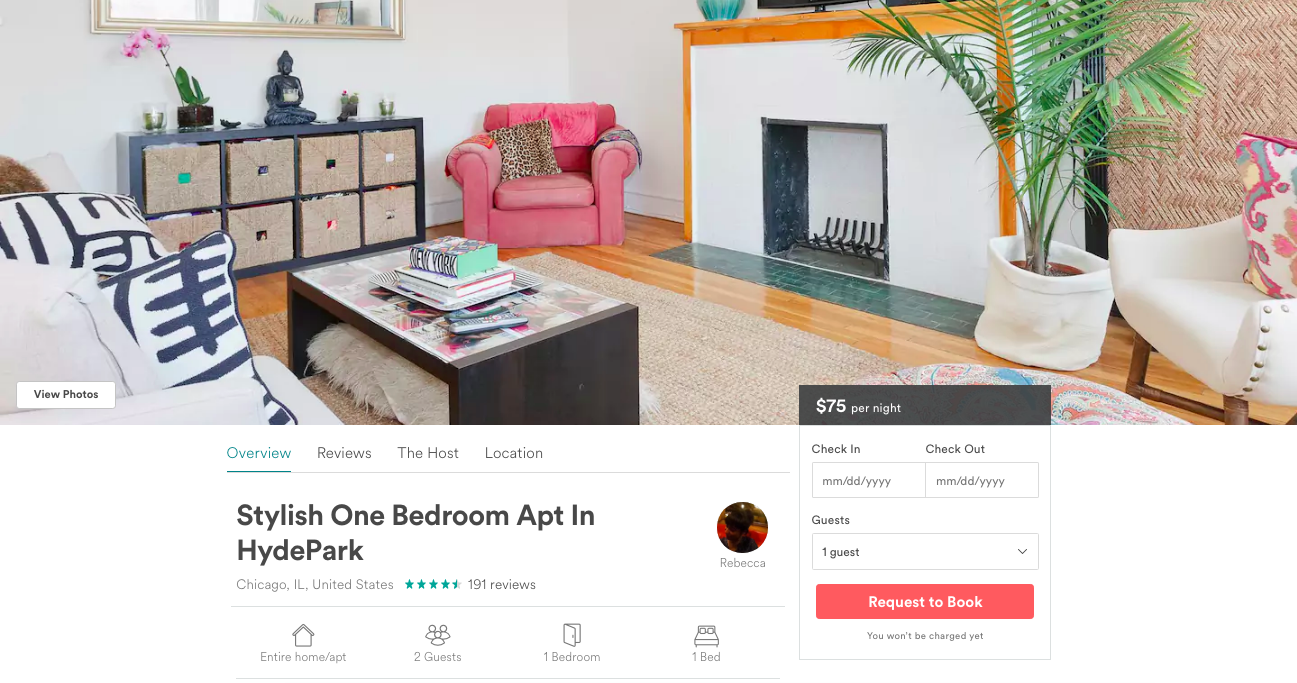
\includegraphics[width=.9\textwidth]{sample1-cover}
\caption{Sample listing profile from Hyde Park, Chicago}
\end{figure}
\begin{figure}
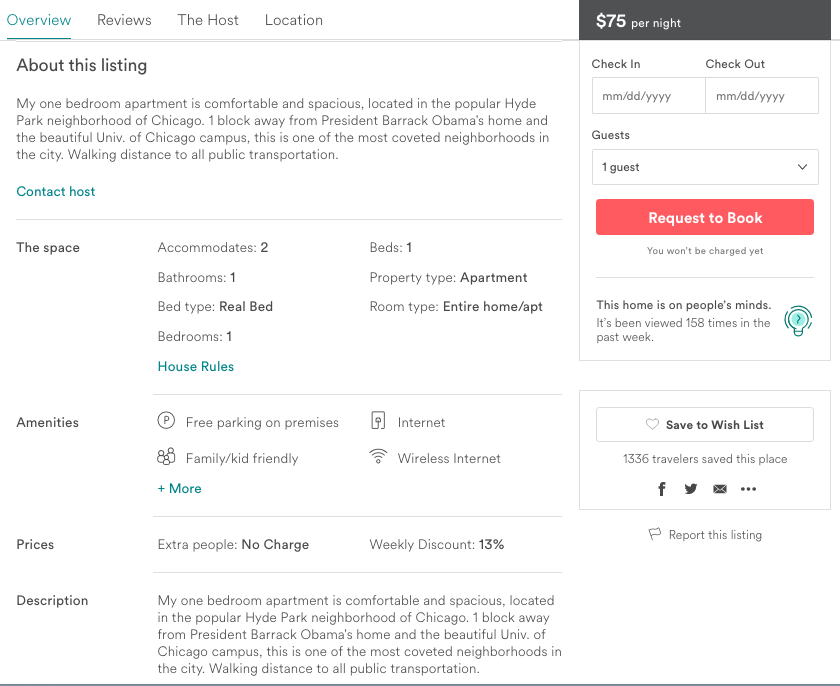
\includegraphics[width=.9\textwidth]{sample2-property}
\caption{Sample property characteristics}
\end{figure}
\begin{figure}

\includegraphics[width=.8\textwidth]{sample3-reviews}
\caption{Sample review information}
\end{figure}
\begin{figure}

\includegraphics[width=.9\textwidth]{sample4-host}
\caption[Sample host information]{Sample host information available. Note that this Figure reflects the changes made to the website after Airbnb updated its discrimination policy. The guests in my data would have seen a larger host profile picture than shown here.}
\end{figure}
\begin{figure}
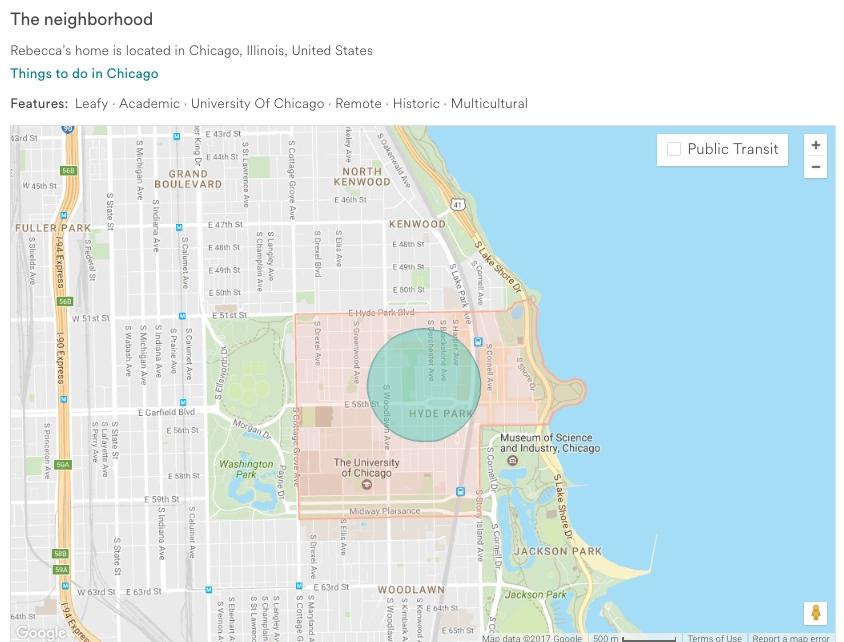
\includegraphics[width=.8\textwidth]{sample5-location}
\caption{Sample location information}
\end{figure}
\begin{figure}
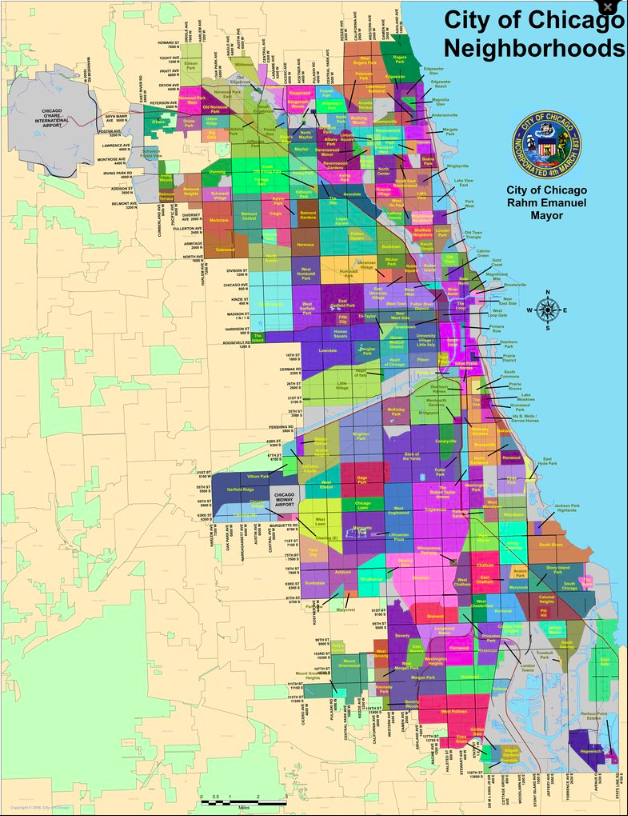
\includegraphics[width=.8\textwidth]{chicago_city_neighborhoods}
\caption[City of Chicago neighborhoods]{City of Chicago neighborhoods, showing level of granularity of neighborhood controls}
\end{figure}


\newpage

\begin{thebibliography}{16} 
\bibitem{sharing}
Frenken, Koen. ``Political Economies and Environmental Futures for the Sharing Economy." Philosophical transactions. Series A, Mathematical, physical, and engineering sciences 375.2095 (2017): 20160367. PMC. Web. 22 July 2017.
\bibitem{rural}
Beyond cities: How Airbnb Supports Rural America?s Revitalization. Rep. Airbnb, 2017. Web. 22 July 2017. Available at: $https://press.atairbnb.com/app/uploads/2017/06/Beyond-Cities_United-States-National-Report.pdf.$ 
\bibitem{elderly}
Airbnb?s Growing Community of 60+ Women Hosts. Rep. Airbnb, 2015. Web. 22 July 2017. Available at: $https://www.airbnbaction.com/wp-content/uploads/2016/03/Airbnb_60_Plus_Women_Report.pdf.$ 
\bibitem{nyt2}
Zipkin, Amy. ``Renting Rooms to Travelers Can Be a Source of Income Later in Life." The New York Times. The New York Times, 17 June 2016. Web. 22 July 2017.
\bibitem{nyt3}
Benner, Katie. ``Airbnb Adopts Rules to Fight Discrimination by Its Hosts." The New York Times. The New York Times, 08 Sept. 2016. Web. 23 Apr. 2017.
\bibitem{oliver}
Oliver, Melvin L., and Thomas M. Shapiro. Black wealth, white wealth: A new perspective on racial inequality. Taylor \& Francis, 2006.
\bibitem{reardon}
Reardon, Sean F., Lindsay Fox, and Joseph Townsend. ``Neighborhood income composition by household race and income, 1990?2009." The Annals of the American Academy of Political and Social Science 660.1 (2015): 78-97.
\bibitem{krysan}
Krysan, Maria, Kyle Crowder, and Michael DM Bader. ``Pathways to residential segregation." Choosing homes, choosing schools (2014): 27-63.
\bibitem{edelman}
Edelman, Benjamin G., and Michael Luca. ``Digital discrimination: The case of Airbnb.com." (2014).
\bibitem{sentimentr}
https://github.com/trinker/sentimentr
\bibitem{aboutus}
``About Us." Airbnb. N.p., n.d. Web. 23 Apr. 2017.
\bibitem{swedenwage}
``Closing the Gender Gap: Act Now." (n.d.): 296. OECD, 17 Dec. 2012. Web. 30 Nov. 2015.
\bibitem{becker}
Becker, Gary S. The Economics of Discrimination. Chicago: U of Chicago, 1957. Print.
\bibitem{bertrand}
Bertrand, Marianne, and Sendhil Mullainathan. ``Are Emily and Greg more employable than Lakisha and Jamal? A field experiment on labor market discrimination." The American Economic Review 94.4 (2004): 991-1013.
\bibitem{doleac}
Doleac, Jennifer, and Luke Stein. ``Race has a hand in determining market outcomes." (2010).
\bibitem{pope}
Pope, Devin G., and Justin R. Sydnor. ``What?s in a Picture? Evidence of Discrimination from Prosper. com." Journal of Human Resources 46.1 (2011): 53-92.
\bibitem{knittel}
Ge, Yanbo, et al. Racial and gender discrimination in transportation network companies. No. w22776. National Bureau of Economic Research, 2016.
\bibitem{edelman2}
Edelman, Benjamin G. and Luca, Michael and Svirsky, Dan, Racial Discrimination in the Sharing Economy: Evidence from a Field Experiment (September 16, 2016). Forthcoming, American Economic Journal: Applied Economics. Available at SSRN: https://ssrn.com/abstract=2701902 or http://dx.doi.org/10.2139/ssrn.2701902
\bibitem{insideairbnb}
Cox, Murray. ``Inside Airbnb. Adding Data to the Debate." Inside Airbnb. N.p., n.d. Web. 23 Apr. 2017.
\bibitem{firebaugh}
Firebaugh, Glenn, and Chad R. Farrell. ``Still large, but narrowing: The sizable decline in racial neighborhood inequality in metropolitan America, 1980?2010." Demography 53.1 (2016): 139-164.
\bibitem{logan}
Logan, John R. ``Separate and unequal: The neighborhood gap for blacks, Hispanics and Asians in Metropolitan America." Project US2010 Report (2011): 1-22.
\bibitem{census}
``U.S. Census Bureau Data". U.S. Census Bureau. 2010. Retrieved 2017-04-22.
\bibitem{hu}
Hu, Minqing, and Bing Liu. ``Mining and summarizing customer reviews." Proceedings of the tenth ACM SIGKDD international conference on Knowledge discovery and data mining. ACM, 2004.
\bibitem{fradkin}
Fradkin, Andrey, Elena Grewal, and David Holtz. The Determinants of Online Review Informativeness: Evidence from Field Experiments on Airbnb. Mimeo, 2017.
\end{thebibliography}

%%Add Fradkin citation



%\bibitem{nyt1}
%Dobbins, James. ``Making a Living With Airbnb." The New York Times. The New York Times, 07 Apr. 2017. Web. 22 July 2017.







\end{document}  